\begin{frame}{Aperiodic Algorithm Review}
  \begin{columns}
  \column{0.48\linewidth}
  \centering
\begin{center}
  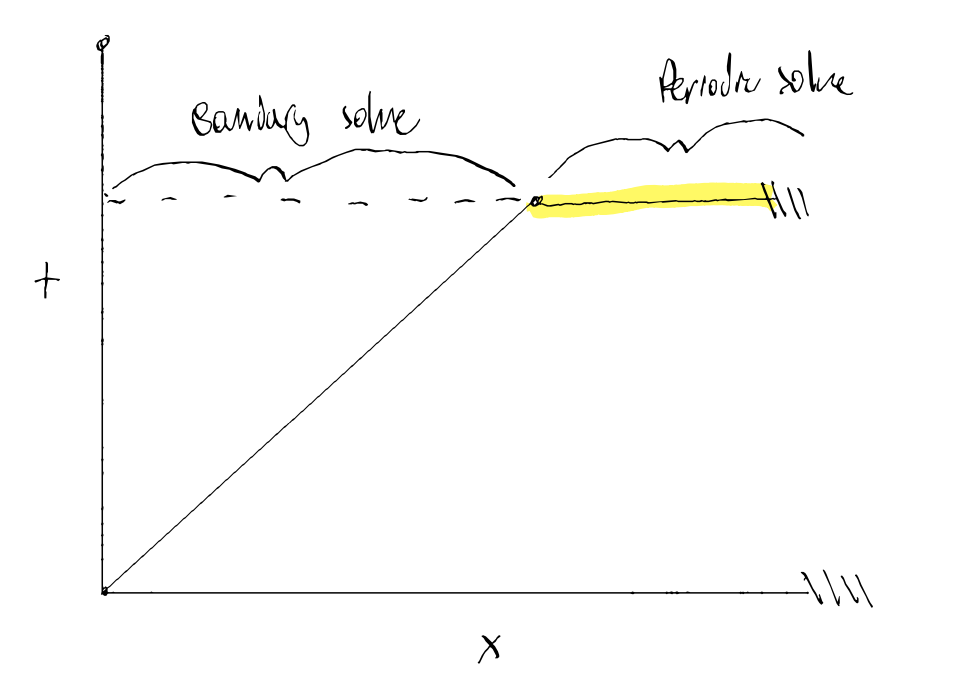
\includegraphics[width=\textwidth]{ap_review_1.png}
  \end{center}

  \column{0.48\linewidth}
  \centering

  \begin{center}
  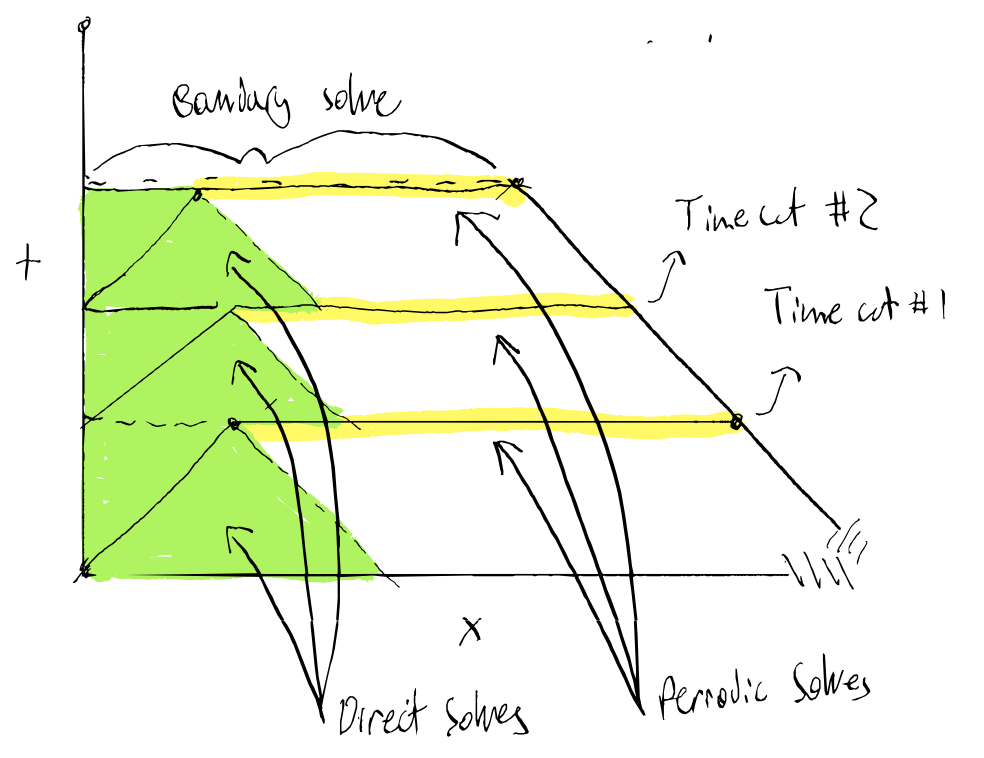
\includegraphics[width=\textwidth]{ap_review_2.png}
  \end{center}
\end{columns}
\end{frame}



\begin{frame}{AP Plan}
  \begin{columns}
  \column{0.38\linewidth}
  \begin{outline}
  \1 A tree structure with three node types:
  \2 Periodic Solve
  \2 Direct Solve
  \2 Special Repeat node for root
  \1 Two kinds of edges:
  \2 Time cuts (red)
  \2 Boundary solves (blue)
  \end{outline}

  \column{0.58\linewidth}
  \begin{center}
  \centering
  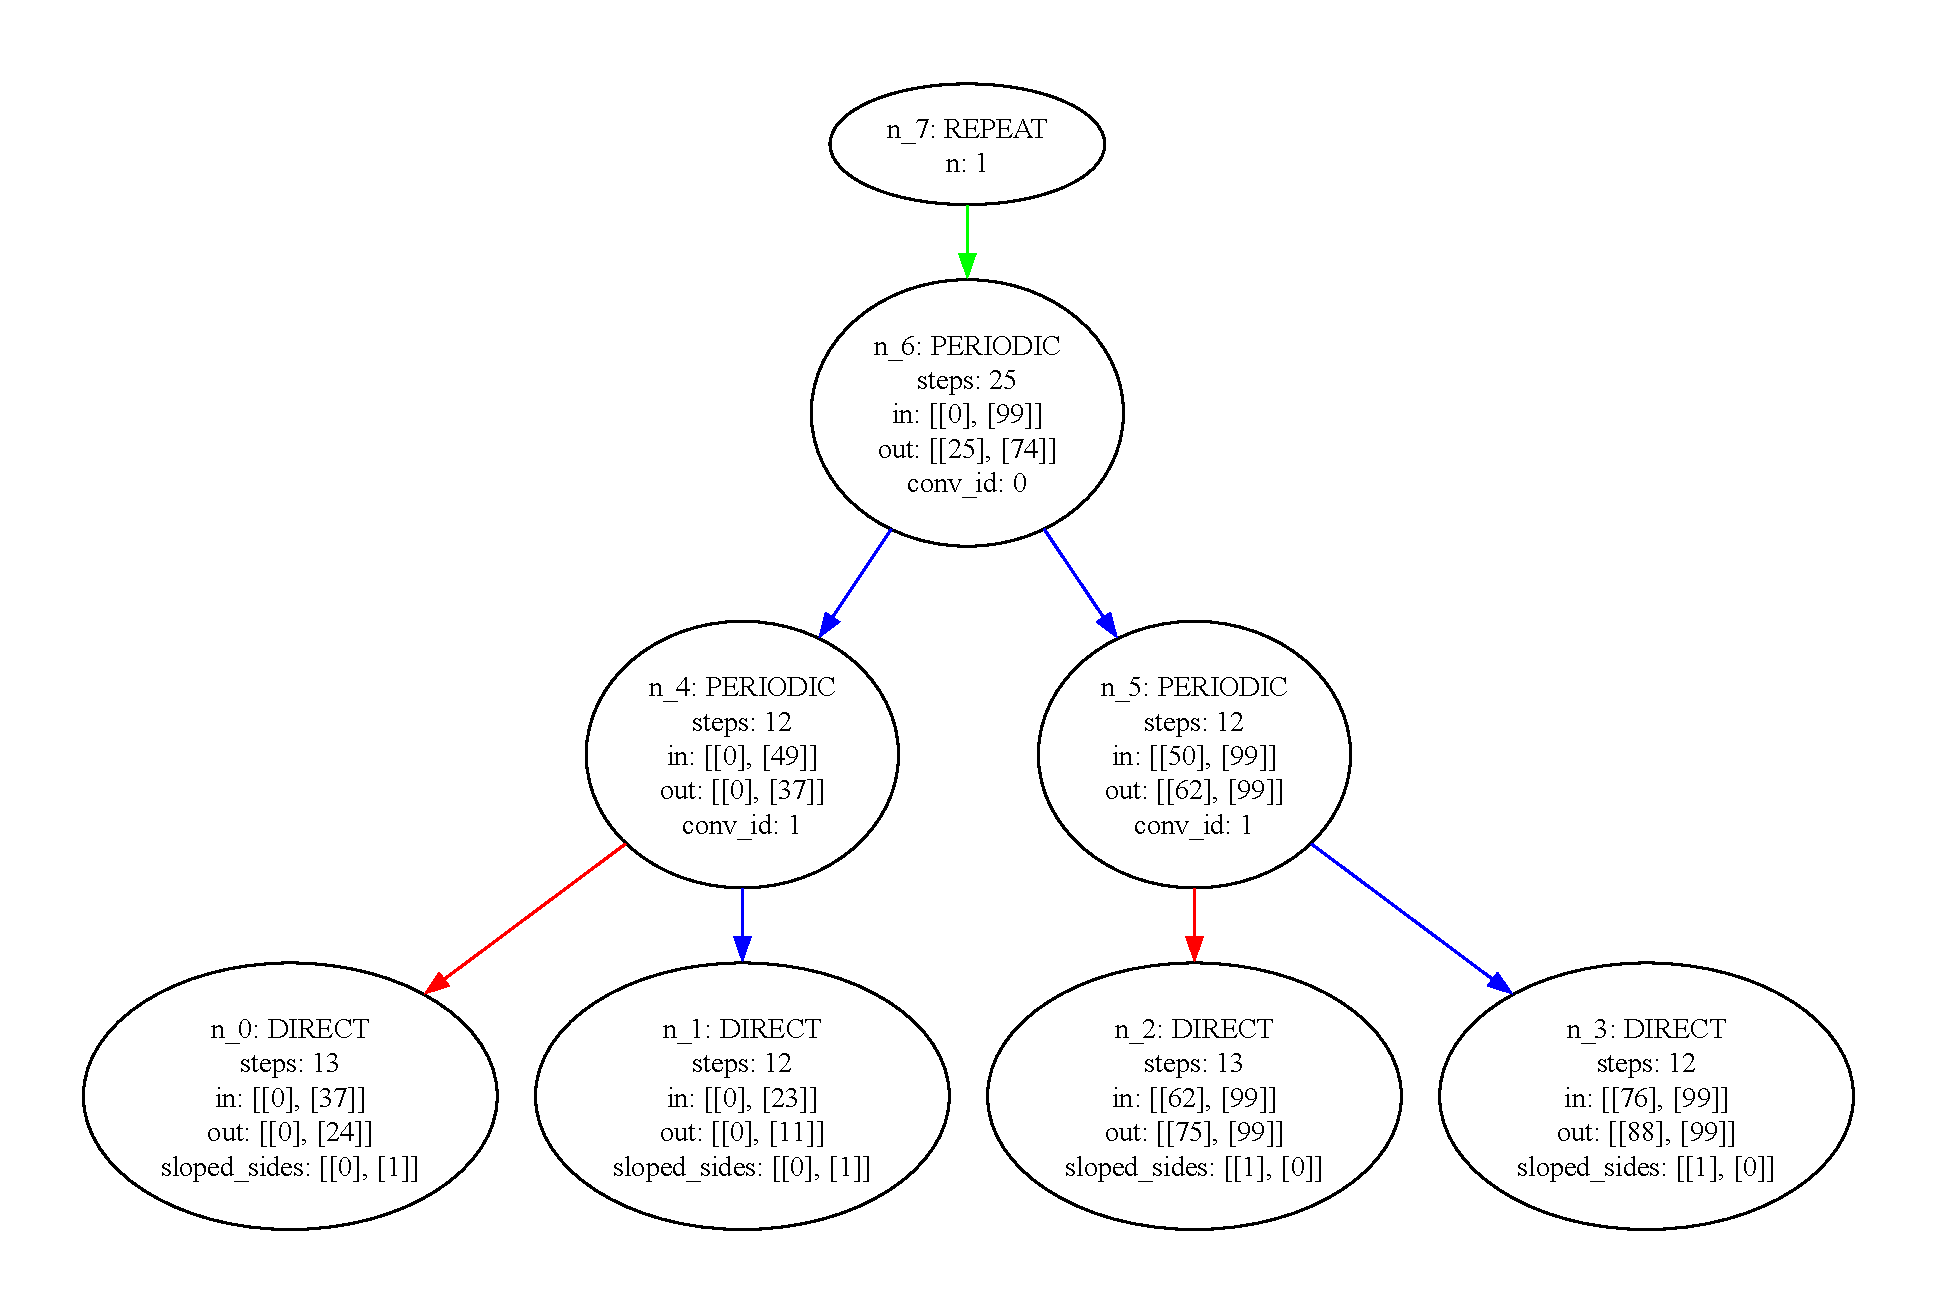
\includegraphics[width=\textwidth]{simple_1d_plan.pdf}
  1D heat, $N = 100$, $\text{steps} = 25$
  \end{center}
\end{columns}
\end{frame}

\begin{frame}{AP Plan: Repeat Node}
  \begin{columns}
  \column{0.38\linewidth}
  \begin{outline}
  \1 Plan is for fixed step count
  \1 Largest periodic solve may not reach step count
  \2 May have to repeat multiple times
  \2 May have remainder leftover
  \end{outline}

  \column{0.58\linewidth}
  \begin{center}
  \centering
  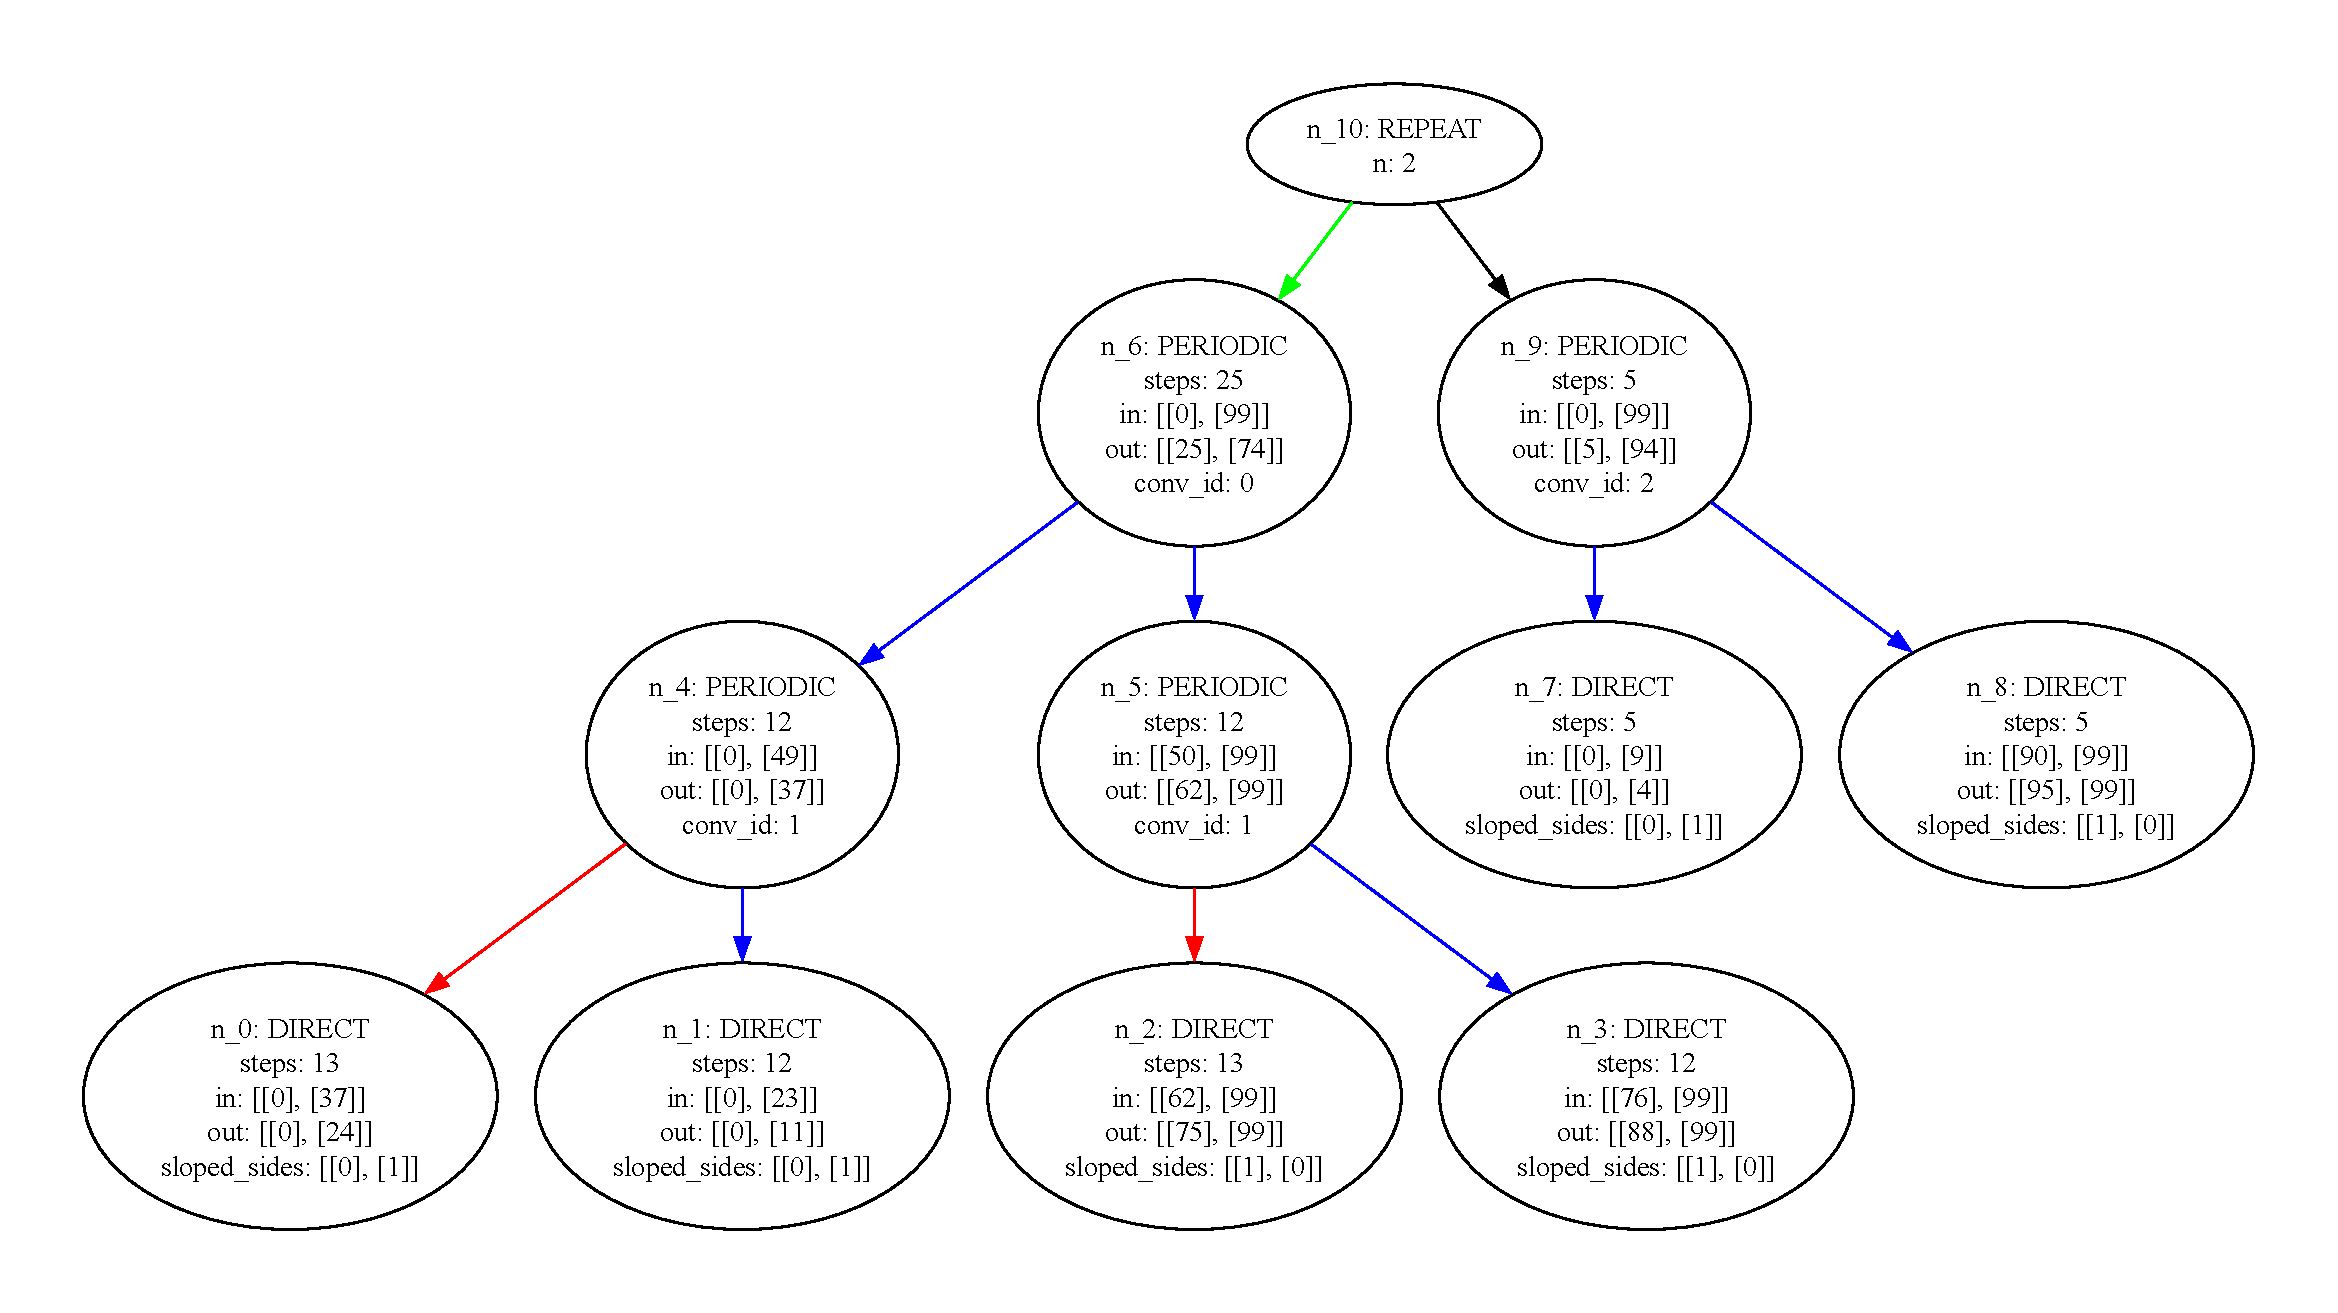
\includegraphics[width=\textwidth]{simple_1d_plan_repeat.pdf}
  1D heat, $N = 100$, $\text{steps} = 55$
  \end{center}
\end{columns}
\end{frame}

\begin{frame}{Finding Periodic Solves}
  \begin{columns}
  \column{0.48\linewidth}
  \begin{outline}
  \1 Two Parameters:
  \1 Cutoff 
  \2 When to switch to direct
  \2 Base case for recursion
  \1 Output Ratio
  \2 Size of output relative to input 
  \2 Determines steps
  \2 Stencil slopes, $\sigma$ are important
  \end{outline}

  \column{0.48\linewidth}
  \begin{center}
  \centering
  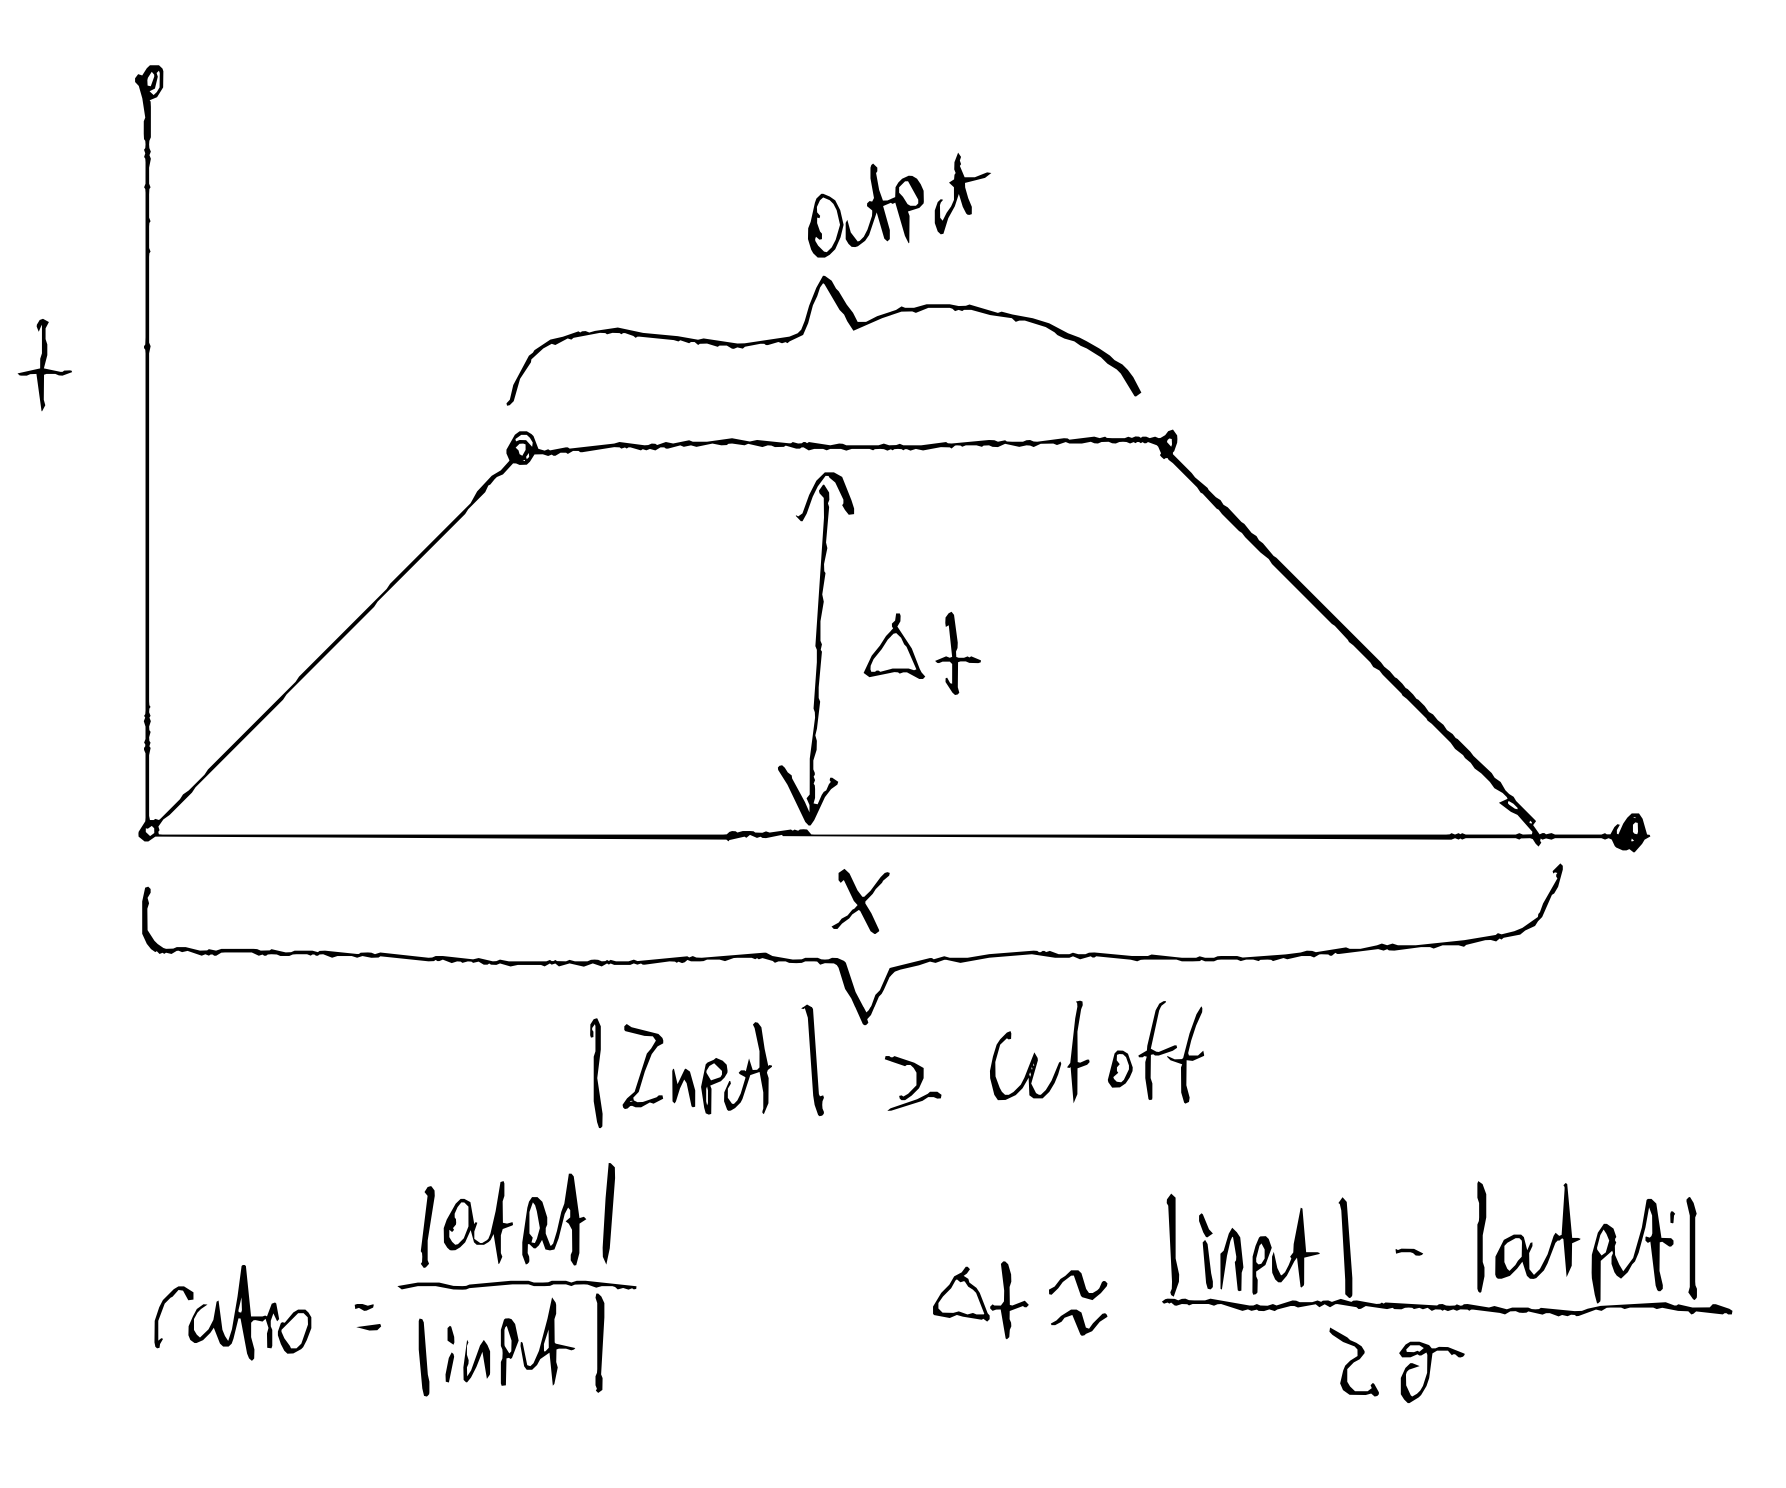
\includegraphics[width=\textwidth]{fft_solve_diagram.png}
  \end{center}
\end{columns}
\end{frame}

\begin{frame}{Central Solve Recursion}
  \begin{columns}
  \column{0.48\linewidth}
  \begin{outline}
  \1 Periodic solve for central region.
  \1 Recursive solves on the boundary
  \1 Works in arbitrary dimension
  \2 Start with axis 0
  \2 Shave off min and max boundary regions
  \2 Repeat for next axis
  \end{outline}

  \column{0.48\linewidth}
  \begin{center}
  \centering
  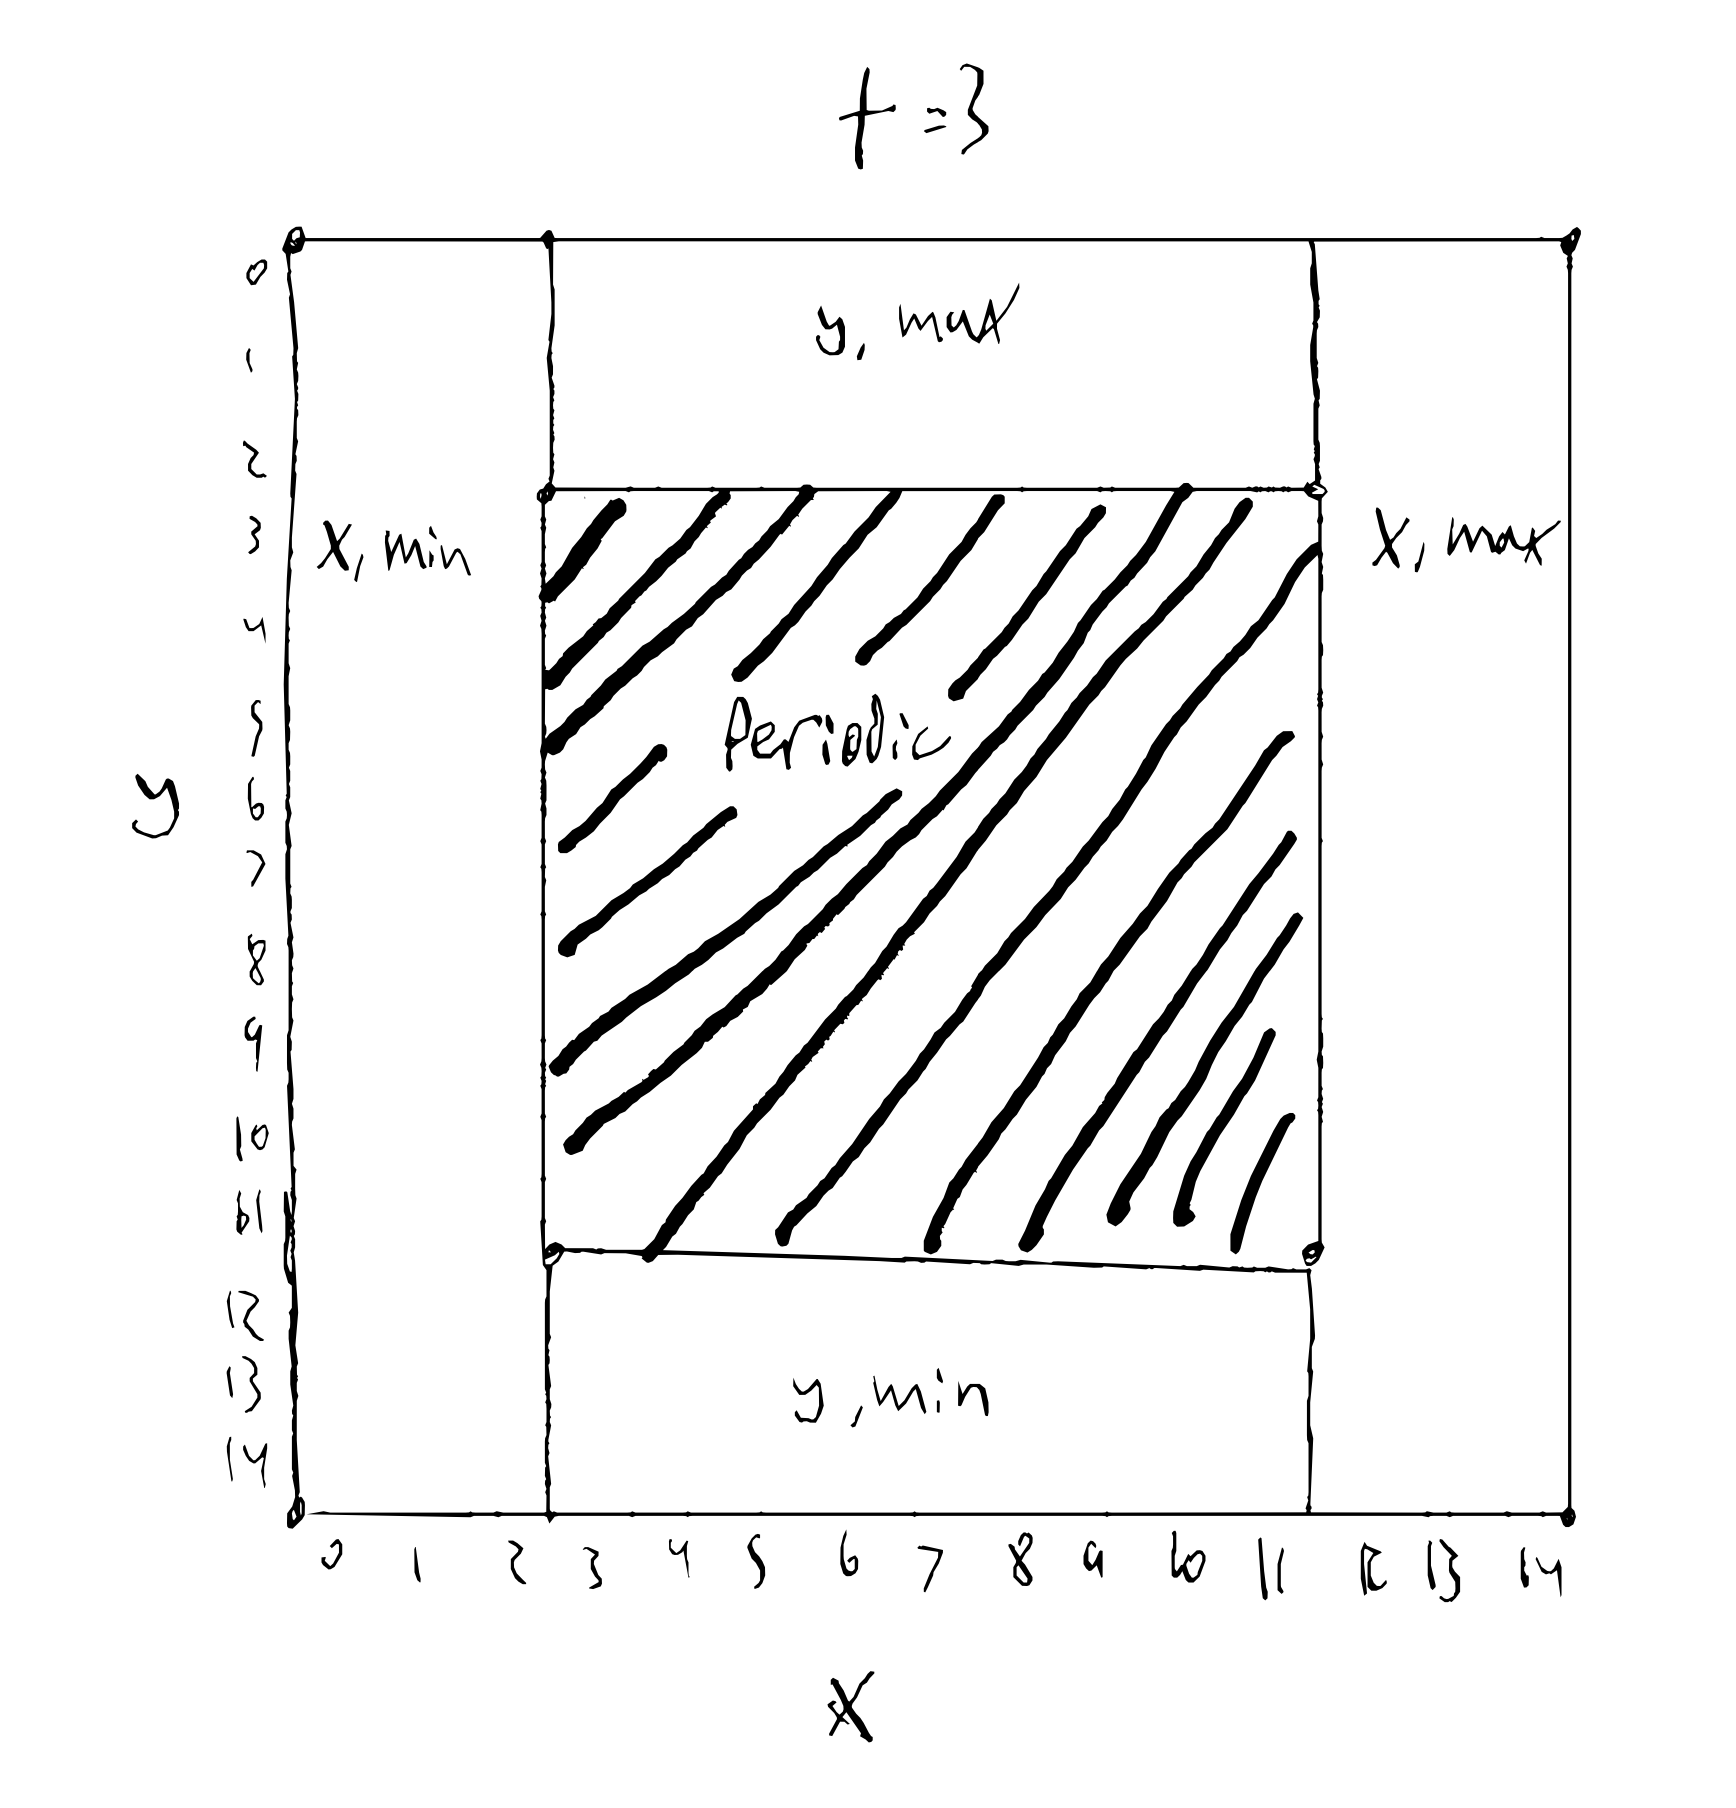
\includegraphics[width=\textwidth]{decomp_2d.png}
  \end{center}
\end{columns}
\end{frame}

\begin{frame}{Frustrums}
  \begin{columns}
  \column{0.48\linewidth}
  \begin{outline}
  \1 Boundary Solves imply volumes of space-time 
  \1 Slopes on the inside
  \1 Flat facing the boundary
  \1 Uniquely defined by
  \2 Output AABB
  \2 Recusion Axis
  \2 Side
  \1 Input AABB depends on stencil radius $\sigma$
  \1 Primary object used to create plans
  \end{outline}

  \column{0.48\linewidth}
  \begin{center}
  \centering
  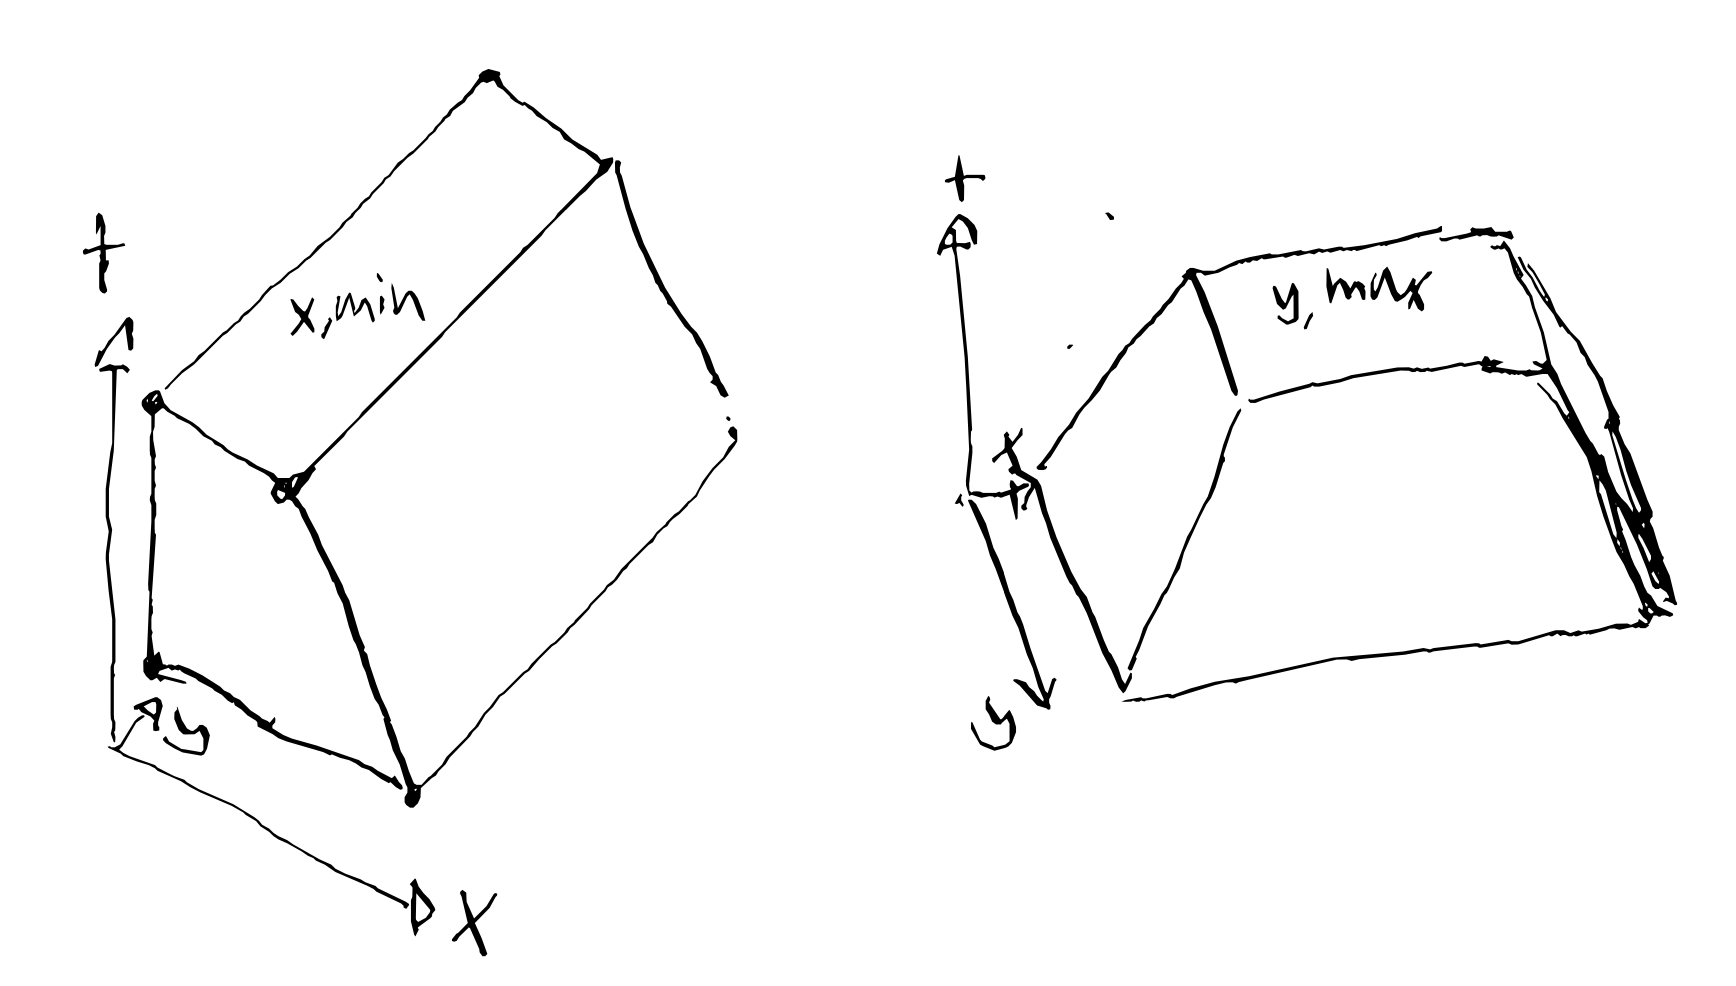
\includegraphics[width=0.8\textwidth]{frustrum_examples.png}

  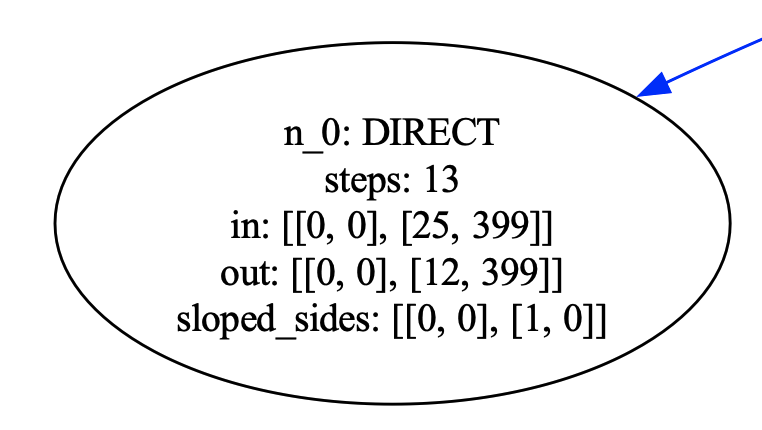
\includegraphics[width=0.5\textwidth]{direct_node.png}
  \end{center}
\end{columns}
\end{frame}

\begin{frame}{Frustrum Recursion}
  \begin{columns}
  \column{0.48\linewidth}
  \begin{outline}
  \1 Periodic solve for portion of output AABB
  \1 Similar to central decomposition 
  \1 Consider axis $A$ 
  \1 Fixed grid dimension $D$
  \1 $2 * (D - A) + 1$ boundary frustrums
  \1 Time-cut frustrums
  \end{outline}

  \column{0.48\linewidth}
  \begin{center}
  \centering
  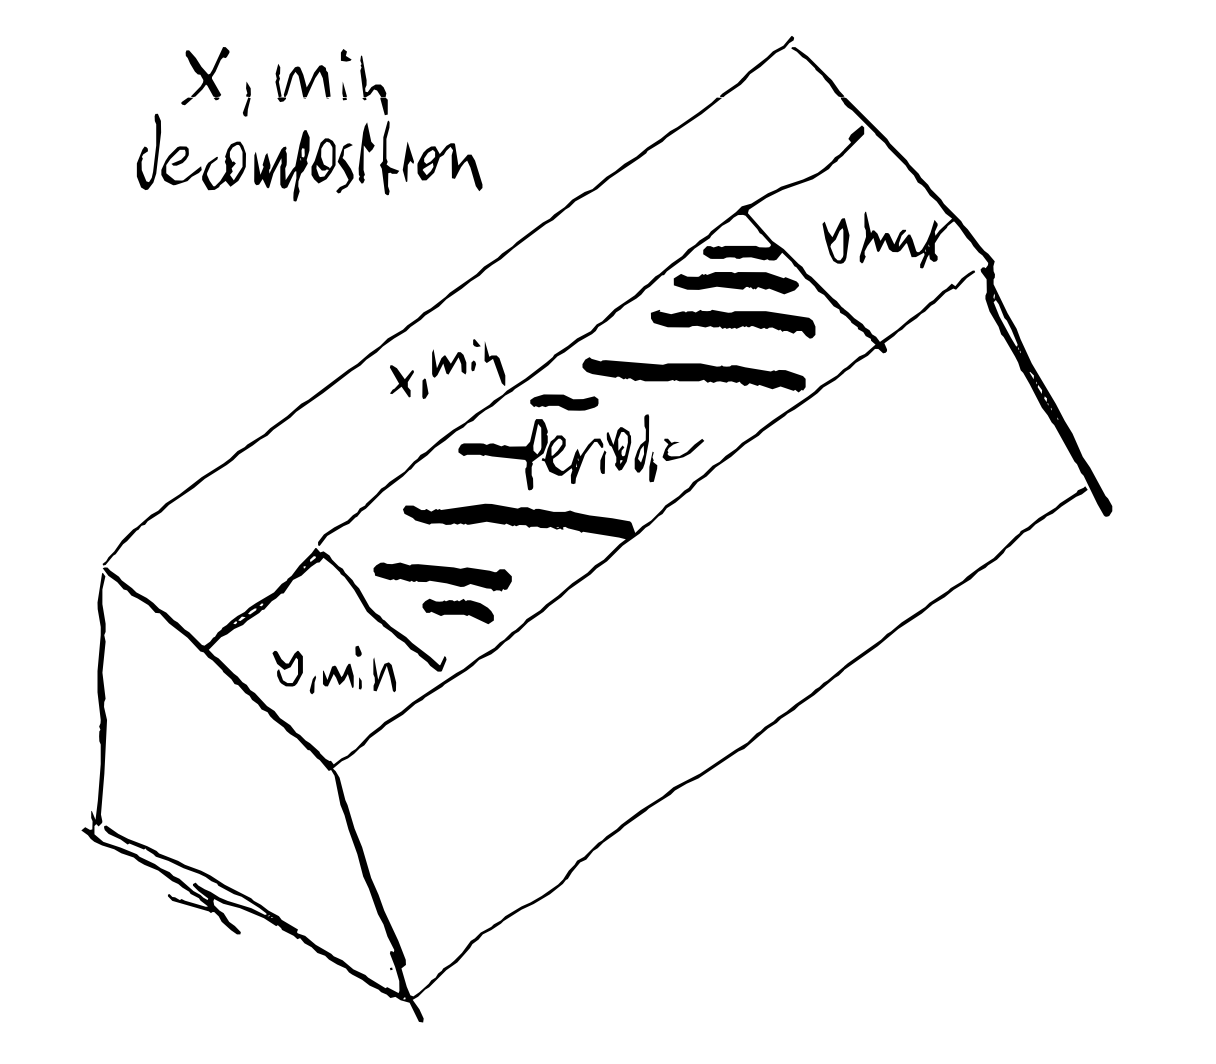
\includegraphics[width=0.6\textwidth]{frustrum_decomp.png}

  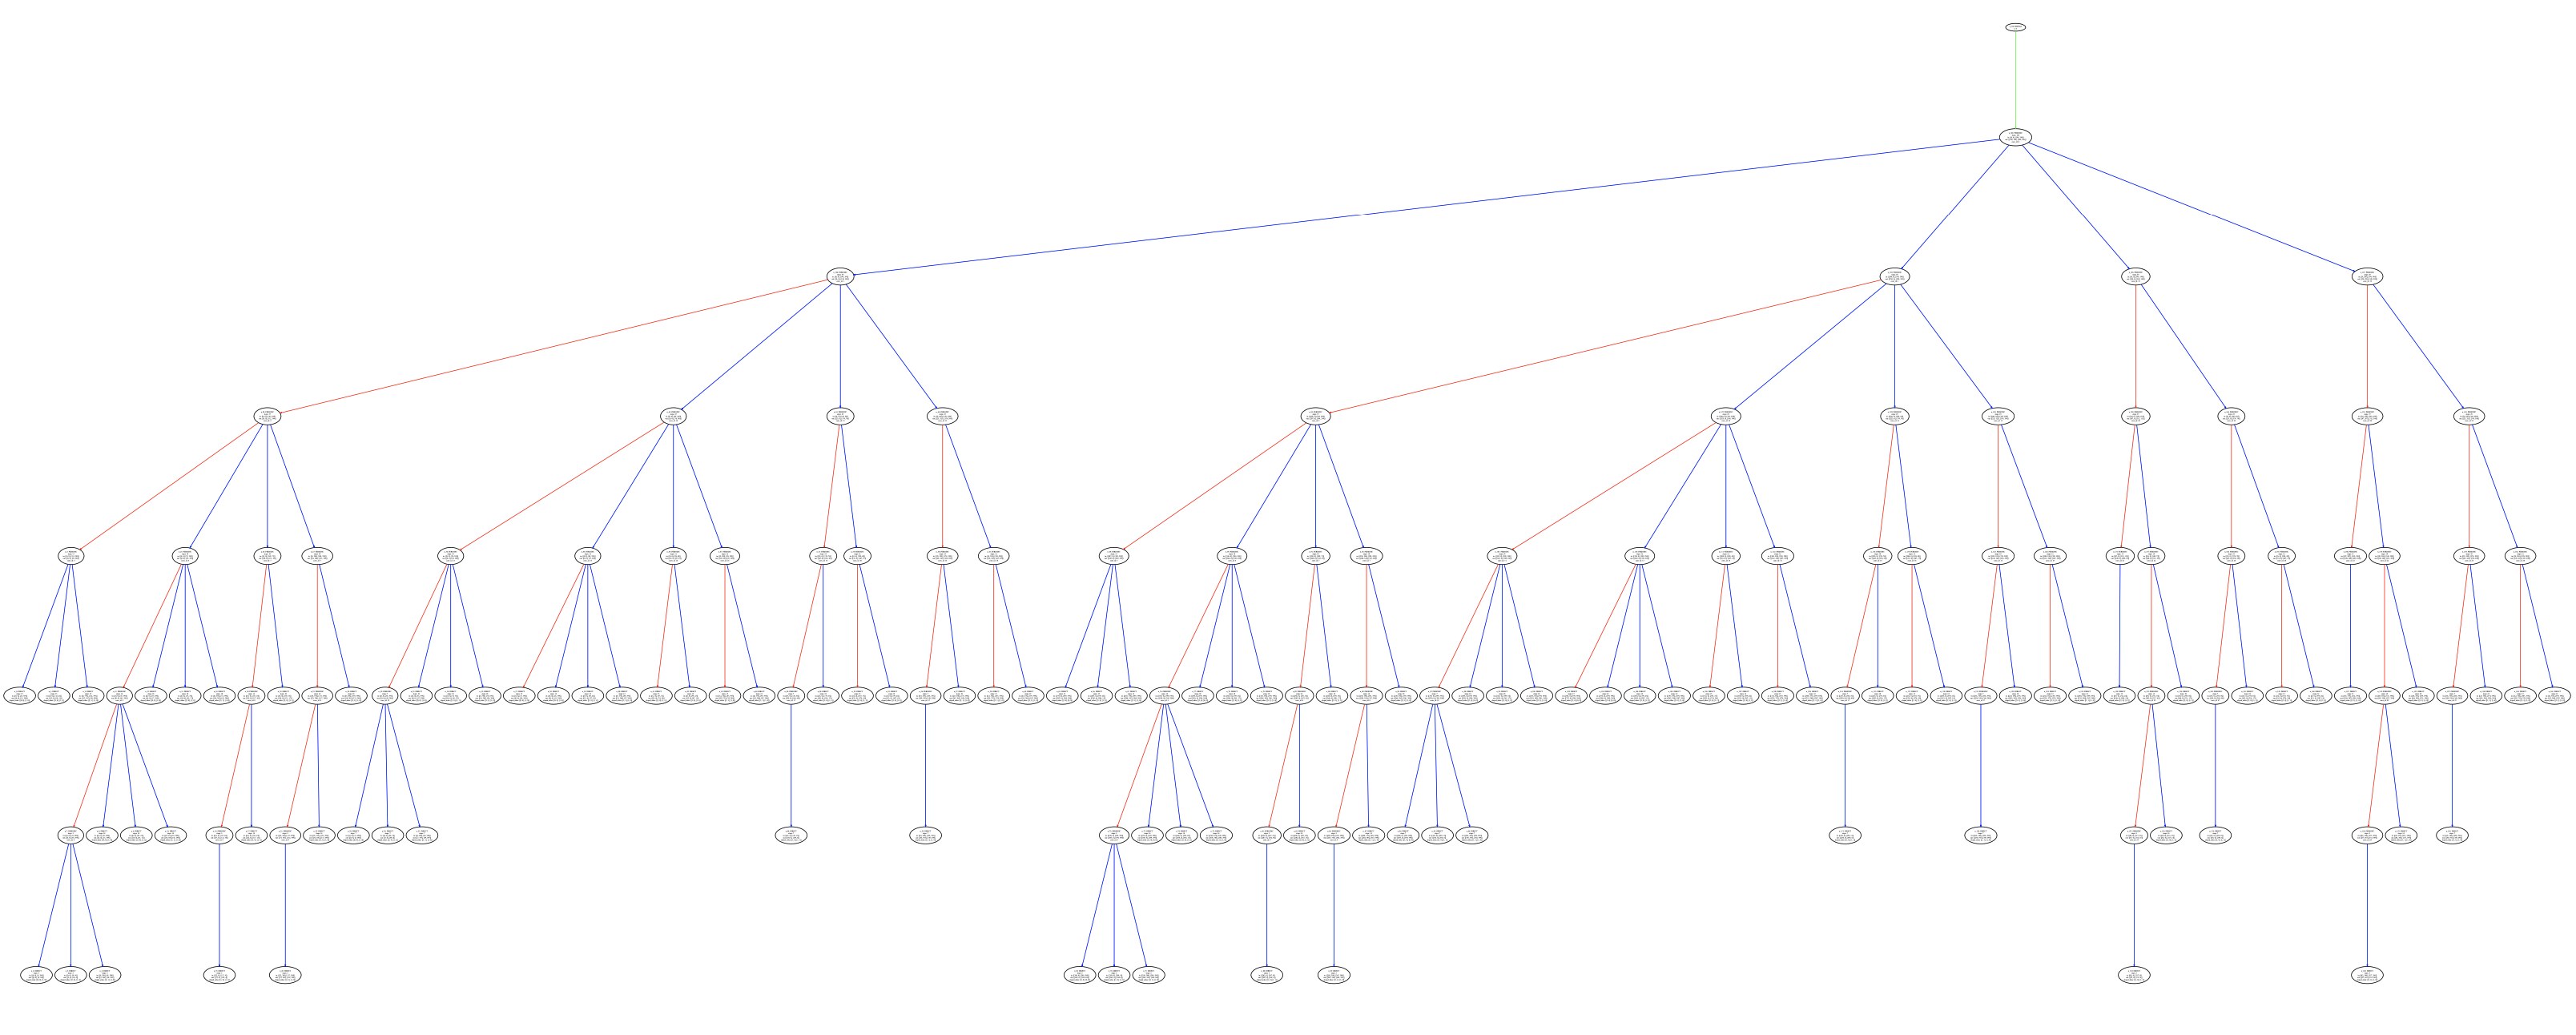
\includegraphics[width=\textwidth]{plan_2d_large.png}
  \end{center}
\end{columns}
\end{frame}
